
\de{ĐỀ THI HỌC KỲ I NĂM HỌC 2022-2023}{THPT Nguyễn Du}



\begin{bt}%[0T3B1-2]%%[Dự án đề kiểm tra HK1 NH22-23 Lê Hùng Thắng]%[Nguyễn Du - tp HCM]
Tìm tập xác định của hàm số $y=\dfrac{\sqrt{1-3x}}{x+5}$.
\loigiai{
Hàm số xác định khi $\heva{&1-3x\ge 0 \\& x+5 \ne 0} \Leftrightarrow \heva{&x\le \dfrac{1}{3}\\ & x \ne -5.}$\\
Vậy tập xác định của hàm số là
$\mathscr{D}=\left(-\infty;\dfrac{1}{3}\right] \setminus \big\{-5\big\}$.
}
\end{bt}

\begin{bt}%[0T3B1-4]%%[Dự án đề kiểm tra HK1 NH22-23 Lê Hùng Thắng]%[Nguyễn Du - tp HCM]
Xác định điều kiện của tham số $m$ để hàm số $y=(3-4m)x-2$ nghịch biến trên $\mathbb{R}$.
\loigiai{
Hàm số nghịch biến trên $\mathbb{R}$ khi $3-4m <0 \Leftrightarrow  m >\dfrac{3}{4}$.
}
\end{bt}

\begin{bt}%[0T3B2-2]%%[Dự án đề kiểm tra HK1 NH22-23 Lê Hùng Thắng]%[Nguyễn Du - tp HCM]
\immini{
Cho hàm số $y=ax^2+bx+2$ $(a \neq 0)$ có đồ thị như hình bên. Hãy xác định các giá trị $a$ và $b$.}
{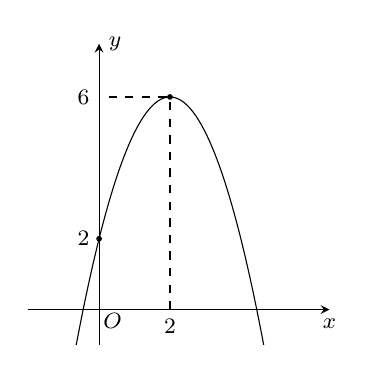
\begin{tikzpicture}[scale=0.45,font=\footnotesize,samples=200,>=stealth]
\draw[->] (-2,0)--(6.5,0) node[below]{$x$};
\draw[->] (0,-1)--(0,7.5) node[right]{$y$};
\node at (0,0) [below right=-2pt]{$O$};
\clip (-1,-1) rectangle (5.1,6.6);
\draw plot[domain=-1:5.1](\x,{-(\x)^2+4*\x+2});
\fill (0,2) circle(2.3pt) node[left]{$2$};
\fill (2,6) circle(2.3pt);
\draw[dashed] (2,0)node[below]{$2$}|-(0,6)node[left]{$6$};
\end{tikzpicture}
}
\loigiai{
Vì đồ thị là Parabol đi qua điểm $(2;6)$ và có trục đối xứng là $x=2$ nên ta có
\[\heva{&\dfrac{-b}{2a}=2 \\& 6=4a+2b+2} \Leftrightarrow \heva{&4a+b=0 \\&4a+2b=4} \Leftrightarrow \heva{&a=-1 \\& b=4.}\]
}
\end{bt}

\begin{bt}%[0T6K1-2]
Nhà sản xuất công bố chiều dài và chiều rộng của một tấm thép hình chữ nhật là $100 \pm 0{,}4 \mathrm{\,cm}$ và $60 \pm 0{,}4 \mathrm{\,cm}$. Tính diện tích của tấm thép.
\loigiai{
Gọi $\overline{a}$ và $\overline{b}$ là chiều dài và chiều rộng thực của tấm thép.\\
Ta có $99{,}6\le \overline{a}\le 100{,}4$ và $59{,}6\le \overline{b}\le 60{,}4$.\\
Suy ra $99{,}6 \cdot 59{,}6 = 5936{,}16 \le \overline{a}\cdot \overline{b}\le 100{,}4 \cdot 60{,}4 =6064{,}16$. \\
Do đó $5936{,}16 -6000 = -64{,}84 \le \overline{a}\cdot \overline{b} -6000 \le 6064{,}14- 6000 =64{,}16$.\\
Vậy diện tích của tấm thép là $6\,000 \pm 64{,}16$ cm$^2$.
}
\end{bt}

\begin{bt}%[0T6B3-1]%[0T6B3-3]%[0T6B3-4]%%[Dự án đề kiểm tra HK1 NH22-23 Lê Hùng Thắng]%[Nguyễn Du - tp HCM]
Kết quả bài thi môn Toán của các bạn học sinh tổ $1$ và tổ $2$ cho ở bảng sau
\begin{longtable}{|c|c|c|c|c|c|c|c|c|c|c|c|c|c|c|c|}
\hline Tổ $1$ & $7$ & $7$ & $6$ & $8$ & $9$ & $7$ & $7$ & $10$ & $9$ & $8$ & $6$ & $8$ & $7$ & $8$ & $9$\\
\hline Tổ $2$ & $10$ & $9$ & $8$ & $9$ & $5$ & $7$ & $8$ & $6$ & $10$ & $7$ & $8$ & $8$ & $9$ & $10$ & $6$\\
\hline
\end{longtable}
\noindent
Hãy tìm số trung bình, tứ phân vị và mốt của kết quả bài thi ở mỗi tổ theo mẫu số liệu trên.
\loigiai{
Kết quả bài thi Toán của các bạn học sinh tổ $1$ và tổ $2$ được sắp xếp lại là
\begin{longtable}{|c|c|c|c|c|c|c|c|c|c|c|c|c|c|c|c|}
	\hline Tổ $1$ & $6$ & $6$ & $7$ & $7$ & $7$ & $7$ & $7$ & $8$ & $8$ & $8$ & $8$ & $9$ & $9$ & $9$ & $10$\\
	\hline Tổ $2$ & $5$ & $6$ & $6$ & $7$ & $7$ & $8$ & $8$ & $8$ & $8$ & $9$ & $9$ & $9$ & $10$ & $10$ & $10$\\
	\hline
\end{longtable} 
\textbf{Xét kết quả của các bạn học sinh tổ $1$ ta có}\\
$\bullet$ Điểm trung bình là $\overline{x}=\dfrac{6\cdot 2+7\cdot 5 +8 \cdot 4 +9 \cdot 3+10}{15}\approx 7{,}7$.\\
$\bullet$ Số trung vị là $M_e=x_8=8$.\\
$\bullet$ Các tứ phân vị là $Q_2=8$; $Q_1=x_4=7$; $Q_3=x_{11}=9$.\\
$\bullet$ Mốt là $M_o=7$.

\textbf{Xét kết quả của các bạn học sinh tổ $2$ ta có}\\
$\bullet$ Điểm trung bình là $\overline{x}=\dfrac{5+6\cdot 2+7\cdot 2 +8 \cdot 4 +9 \cdot 3+10\cdot 3}{15}=8$.\\
$\bullet$ Số trung vị là $M_e=x_8=8$.\\
$\bullet$ Các tứ phân vị là $Q_2=8$; $Q_1=x_4=7$; $Q_3=x_{11}=9$.\\
$\bullet$ Mốt là $M_o=8$.
}
\end{bt}

\begin{bt}%[0T6B4-2]%%[Dự án đề kiểm tra HK1 NH22-23 Lê Hùng Thắng]%[Nguyễn Du - tp HCM]
Kết quả bài thi môn Toán của các bạn học sinh tổ $1$ và tổ $2$ cho ở bảng sau
\begin{longtable}{|c|c|c|c|c|c|c|c|c|c|c|c|c|c|c|c|}
\hline Tổ $1$ & $7$ & $7$ & $6$ & $8$ & $9$ & $7$ & $7$ & $10$ & $9$ & $8$ & $6$ & $8$ & $7$ & $8$ & $9$\\
\hline Tổ $2$ & $10$ & $9$ & $8$ & $9$ & $5$ & $7$ & $8$ & $6$ & $10$ & $7$ & $8$ & $8$ & $9$ & $10$ & $6$\\
\hline
\end{longtable}
\noindent
Hãy tìm phương sai và độ lệch chuẩn kết quả bài thi của mỗi tổ từ đó so sánh độ ổn định kết quả bài thi của $2$ tổ.
\loigiai{
$\bullet$ Phương sai kết quả bài thi của các học sinh tổ $1$ là\\
$S_1^2=\dfrac{1}{15}\left(2\cdot 6^2 + 5\cdot 7^2 + 4\cdot 8^2+ 3\cdot 9^2+ 1\cdot 10^2\right) - 7{,}7^2 \approx 1{,}26$.\\
$ \Rightarrow $ Độ lệch chuẩn là $S_1=\sqrt{S_1^2}\approx 1{,}12$.\\
$\bullet$ Phương sai kết quả bài thi của các học sinh tổ $2$ là\\
$S_2^2=\dfrac{1}{15}\left(1 \cdot 5^2 +2\cdot 6^2 + 2\cdot 7^2 + 4\cdot 8^2+ 3\cdot 9^2+ 3\cdot 10^2\right) - 8^2 \approx 2{,}27$.\\
$ \Rightarrow $ Độ lệch chuẩn là $S_2=\sqrt{S_2^2}\approx 1{,}51$.\\
$\bullet$ Vì $S_1<S_2$ nên kết quả bài thi của các học sinh của tổ $1$ đồng đều hơn.
}
\end{bt}

%Bài 6...........................
\begin{bt}%[0T4B2-1]%[Dự án đề kiểm tra HKI NH22-23- Thành Đức Trung]%[THPT Nguyễn Du - Hồ Chí Minh]
Tính góc lớn nhất của tam giác $ABC$, biết các cạnh là $a=8$, $b=12$ và $c=5$.
\loigiai
{Cạnh lớn nhất của tam giác $ABC$ là cạnh $AC=b=12$ nên góc lớn nhất trong tam giác $ABC$ là góc $\widehat{ABC}$.\\
Áp dụng hệ quả của định lý cô-sin trong tam giác $ABC$ ta có
\[\cos\widehat{ABC}=\dfrac{AB^2+BC^2-AC^2}{2\cdot AB\cdot BC}=\dfrac{5^2+8^2-12^2}{2\cdot5\cdot8}=-\dfrac{11}{16}\Rightarrow\widehat{ABC}\approx133{,}43^{\circ}.\]
Vậy góc lớn nhất của tam giác $ ABC $ xấp xỉ $143{,}33^{\circ}$.
}
\end{bt}

%Bài 7...........................
\begin{bt}%[0T5B3-4]%[Dự án đề kiểm tra HKI NH22-23- Thành Đức Trung]%[THPT Nguyễn Du - Hồ Chí Minh]
Cho tam giác $ABC$, các điểm $M$, $N$ thỏa mãn $\overrightarrow{MB}=\dfrac{1}{2}\overrightarrow{BC}$, $\overrightarrow{AN}=3\overrightarrow{NB}$. Hãy biểu thị $\overrightarrow{MN}$ theo hai véc-tơ $\overrightarrow{AB}$ và $\overrightarrow{BC}$.
\loigiai
{Do $\overrightarrow{AN}=3\overrightarrow{NB}$ nên $\overrightarrow{BN}=-\dfrac{1}{4}\overrightarrow{AB}$.\\
Ta có 
\[\overrightarrow{MN}=\overrightarrow{MB}+\overrightarrow{BN}=\dfrac{1}{2}\overrightarrow{BC}-\dfrac{1}{4}\overrightarrow{AB}.\]
Vậy $\overrightarrow{MN}=\dfrac{1}{2}\overrightarrow{BC}-\dfrac{1}{4}\overrightarrow{AB}$.
}
\end{bt}

%Bài 8...........................
\begin{bt}%[0T5K4-7]%[Dự án đề kiểm tra HKI NH22-23- Thành Đức Trung]%[THPT Nguyễn Du - Hồ Chí Minh]
\immini{
Cho ba lực $\overrightarrow{F_1} = \overrightarrow{MA}$, $\overrightarrow{F_2} = \overrightarrow{MB}$ và $\overrightarrow{F_3} = \overrightarrow{MC}$ cùng tác động vào một vật tại điểm $M$ và vật đứng yên. Cho biết độ lớn của $\overrightarrow{F_1}$, $\overrightarrow{F_2}$ đều bằng $90$ N và góc $\widehat{AMB} = 60^\circ$. Tính độ lớn của lực $\overrightarrow{F_3}$.
}{
\begin{tikzpicture}[scale=.8, font=\footnotesize, line join=round, line cap=round, >=stealth]
\path
(0,0)coordinate(M)
(-4.5,0)coordinate(C)
(2.5,1.8)coordinate(A)
(2.5,-1.8)coordinate(B)
;
\draw[->] (M)--(C) node[midway,above]{$\overrightarrow{F_3}$};
\draw[->] (M)--(A) node[midway,above]{$\overrightarrow{F_1}$};
\draw[->] (M)--(B) node[midway,below]{$\overrightarrow{F_2}$};
\foreach \x/\g in{A/0, B/0, C/-180, M/-120}
\fill[black](\x)circle(1pt)($(\x)+(\g:3mm)$)node{$\x$};
\end{tikzpicture}
}
\loigiai{
Vì vật đứng yên nên ta có $\overrightarrow{F_1} + \overrightarrow{F_2} + \overrightarrow{F_3} = \overrightarrow{0} \Leftrightarrow \overrightarrow{F_1} + \overrightarrow{F_2} = -\overrightarrow{F_3}$.\\
Bình phương hai vế và biến đổi ta được
\[
\begin{aligned}
&\left(\overrightarrow{F_1} + \overrightarrow{F_2} \right)^2= \left(-\overrightarrow{F_3}\right)^2\\
\Leftrightarrow\; & \overrightarrow{F_1}^2 + \overrightarrow{F_2}^2 + 2\cdot\overrightarrow{F_1}\cdot\overrightarrow{F_2} = \overrightarrow{F_3}^2 \\
\Leftrightarrow\; & 90^2 + 90^2 + 2\cdot90\cdot90\cdot\cos\widehat{AMB} = \overrightarrow{F_3}^2\\
\Leftrightarrow\; &\overrightarrow{F_3}^2 = 24300 \\
\Leftrightarrow\; & \left|\overrightarrow{F_3}\right| = 90\sqrt{3}.
\end{aligned}
\]
Vậy độ lớn của lực $\overrightarrow{F_3}$ bằng $90\sqrt{3}$ N.
}
\end{bt}

%Bài 9...........................
\begin{bt}%[0T5B4-3]%[Dự án đề kiểm tra HKI NH22-23- Thành Đức Trung]%[THPT Nguyễn Du - Hồ Chí Minh]
Cho hình chữ nhật $ABCD$ có tâm $O$ và cho $AB = 3a$, $AD = 4a$. Tính $\overrightarrow{AB}\cdot\overrightarrow{AO}$.
\loigiai
{
\immini{
Ta có
\[
\begin{aligned}
\overrightarrow{AB}\cdot\overrightarrow{AO} &= \overrightarrow{AB}\cdot\dfrac{1}{2}\overrightarrow{AC}\\
&=\overrightarrow{AB}\cdot\dfrac{1}{2}\left(\overrightarrow{AB} + \overrightarrow{AD}\right) \\
&= \dfrac{1}{2}\cdot AB^2 + \dfrac{1}{2}\cdot\overrightarrow{AB}\cdot\overrightarrow{AD}\\
&= \dfrac{1}{2}\cdot\left(3a\right)^2\quad\left(\text{vì}\;\overrightarrow{AB}\perp\overrightarrow{AD}\;\text{nên}\;\overrightarrow{AB}\cdot\overrightarrow{AD}=0\right)\\
&=\dfrac{9a^2}{4}.
\end{aligned}
\]
}{
\begin{tikzpicture}[scale=1, font=\footnotesize, line join=round, line cap=round, >=stealth]
\path
(0,0)coordinate(A)
(3,0)coordinate(B)
(3,-4)coordinate(C)
(0,-4)coordinate(D)
(1.5,-2)coordinate(O)
;
\draw(A)--(B)--(C)--(D)--(A)--(C) (B)--(D);
\draw (A)--(B) node[midway,above]{$3a$};
\draw (A)--(D) node[midway,left]{$4a$};
\foreach \x/\g in{A/90, B/90, C/-90, D/-90, O/90}
\fill[black](\x)circle(1pt)($(\x)+(\g:3mm)$)node{$\x$};
\end{tikzpicture}
}
}
\end{bt}